Tracks A and B measure the same ten systems, in the same indexing mode, over the same corpora. They do not agree, and the disagreement falls where the mechanism predicts. On \textit{Fann or Flop}, BM25 ranks first of ten on Track A and last of ten on Track B, a shift of nine places (Figure~\ref{fig:dissoc}). No other system moves more than four. On \textit{Diwan}, where queries carry no remembered wording, BM25 is poor under both protocols and the ranks broadly agree. The dissociation is a property of the tip-of-the-tongue regime, not of BM25 in general.

Correlating the two rankings gives Kendall $\tau{=}+0.24$ ($p{=}0.38$) on \textit{Fann or Flop}
against $\tau{=}+0.51$ ($p{=}0.047$) on \textit{Diwan}. We do not read the first as evidence that
the protocols are unrelated in general: with ten systems one outlier is enough to move $\tau$, and
removing BM25 restores agreement ($\tau{=}+0.56$, $p{=}0.045$). Among dense encoders the protocols
largely concur; what dissociates is the lexical system, and only where remembered wording lets
surface matching succeed without any notion of aboutness.

The two results are consistent. Track A rewards recovering a specific remembered item, and where the query carries the item's wording, surface matching is close to sufficient. Track B asks whether retrieved poems are about a theme that is never stated in the poems' own words, and there surface matching has nothing to work with. Both protocols are valid, but they measure different things, and a system's score under one carries little information about its score under the other.

Reporting a single protocol can therefore mislead. A study that evaluated only known-item retrieval on a tip-of-the-tongue query set would conclude that dense retrieval is not worth its cost for Arabic poetry, since a bag of words beats a state-of-the-art 8B encoder. A study that evaluated only thematic relevance would conclude the opposite, with BM25 last of ten and significantly behind eight of the nine dense encoders. Each conclusion is supported by its own data, and neither holds in general.

\begin{figure}[t]
\centering
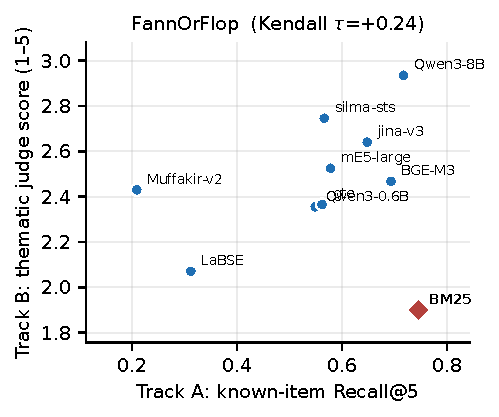
\includegraphics[width=\columnwidth]{figures/fig_dissociation_a.pdf}\\[6pt]
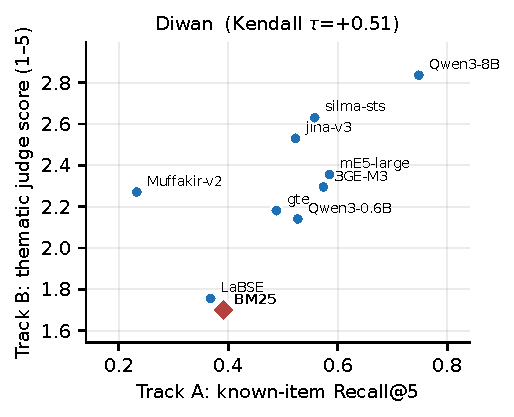
\includegraphics[width=\columnwidth]{figures/fig_dissociation_b.pdf}
\caption{The dissociation. Each point is a system; $x$ is known-item Recall@5, $y$ is the thematic
judge score. Top: on \textit{Fann or Flop}, BM25 (red diamond) is the best system on one axis and
the worst on the other. Bottom: on \textit{Diwan}, where no query carries remembered wording, the
two protocols broadly agree.}
\label{fig:dissoc}
\end{figure}
